\section{Lecture 19}
\subsection{Lecture Notes - Principle Axes of Inertia \& Euler's Equations}
\subsubsection{Motivation Clickers}
Suppose we calculate a diagonal inertia matrix for an objecct in some coordinate system, with $\lambda_1 > \lambda_2 > \lambda_3$. What are the principle axes?
\begin{s}
$(1, 0, 0)$, $(0, 1, 0)$ and $(0, 0, 1)$. If we calculate the inertia matrix to be diagonal in our coordinate system, then it is just the x/y/z axis that are the principal axes. In general, the principal axes are just the coordinate axes if $\II$ is diagonal!
\end{s}
Next, suppose we calculate the moment of inertia of a second object, and it is not diagonal. What are the principle axes in this case?
\begin{s}
$(\v{e}_1, \v{e}_2, \v{e}_3)$ where $\v{e}_i$ are the eigenvectors of $\II$.
\end{s}

\subsubsection{Linear algebra review}
A real symmetric (nxn) matrix can be diagonalized, i.e.:
\[S^{-1}AS = \m{\lambda_1 &  \cdots &  0 \\ \vdots & \ddots & \vdots \\ 0 & \cdots & \lambda_n}\]
The matrix A has eigenvectors $\v{v}_1, \cdots \v{v}_n$ corresponding to eigenvalues $\lambda_1, \cdots \lambda_n$. 

The matrix $S$ has the eigenvectors as its columns, that is, $S = [\v{v}_1, \cdots \v{v}_n]$. 

The eigenvectors obey the equation $A\v{v}_i = \lambda_i\v{v}_i$. 

The eigenvectors form an orthonormal basis. 

Note that $S$ here is an orthogonal matrix, that is, $S^T = S^{-1}$, or $SS^T = SS^{-1} = I$. So we could write the above equivalently as $S^{T}AS$. 

Another property is that $\det S = \pm 1$.


A group theoretic property is that Orthogonal matrices with $\det(S) = 1$ form the $SO(n)$ group.
\newline Multiplication of a vector by a matrix $A$ is a linear transformation $\v{v} \mapsto A\v{v}$. What happens to an eigenvector of $A$ under this linear transformation?
\begin{s}
The magnitude of the vector can change (in fact, it is rescaled by the corresponding eigenvalue) but the direction does not change.
\end{s}
The eigenvalue equation can be written as $(A - \lambda I)\v{v} = \v{0}$. What condition must be satisfied for $\lambda$ to be an eigenvalue of $A$?
\begin{s}
$\det(A - \lambda I) = 0$
\end{s}
The matrix A has eigenvectors $\v{v}_1, \cdots \v{v}_n$ corresponding to eigenvalues $\lambda_1, \cdots \lambda_n$. The matrix $S$ has the eigenvectors as its columns, that is, $S = [\v{v}_1, \cdots \v{v}_n]$. What is the product $AS$?
\begin{s}
Recall that:
\[S^{-1}AS = \m{\lambda_1 &  \cdots &  0 \\ \vdots & \ddots & \vdots \\ 0 & \cdots & \lambda_n}\]
Hence:
\[AS = S\m{\lambda_1 &  \cdots &  0 \\ \vdots & \ddots & \vdots \\ 0 & \cdots & \lambda_n}\]
Therefore the answer is:
\[AS = [\lambda_1 \v{v}_1 \cdots \lambda_n\v{v}_n]\]
\end{s}
(Question from last day) Which of the following statements are a consequence of the fact that the inertia tensor is a 3x3 matrix with real positive eigenvalues and orthogonal eigenvectors?
\begin{enumerate}
    \item The matrix can be diagonalized
    \item The matrix of eigenvectors is an orthogonal matrix
    \item The matrix of eigenvectors is a rotation matrix (if properly normalized)
    \item In the coordinate system aligned with the eigenvectors, the tensor is diagonal.
\end{enumerate}
\begin{s}
    All 4 are correct (for (c), recall that when we diagonalize a matrix, we rotate our axes/coordinate system). 
\end{s}

\subsubsection{Rotational motion and principal axes}
\begin{center}
    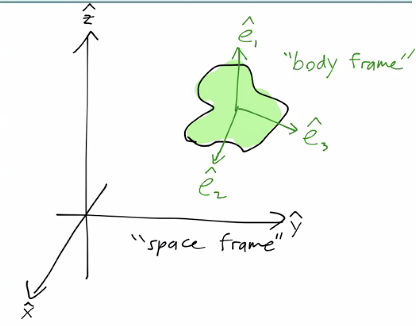
\includegraphics[scale=1]{Lecture-19/l19-img1.png}
\end{center}
We have that the torque is defined as:
\[\bm{\Gamma} = \dot{\v{L}}\]
Where $\bm{\Gamma} = \v{r} \times \v{F}$. We can expand out the time derivative of the angular momentum with:
\[\dot{\v{L}} = \dot{\II}\bm{\omega} + \II\dot{\bm{\omega}}\]
But it is quite nasty to work in a frame where the inertia tensor is constantly changing. Hence, let us work in a coordinate system where $\II$ is fixed and hence $\dot{\II} = 0$. 
\newline How is the time derivative of a vector $\v{v}$ in an inertial frame I related to the time derivative of the vector in a rotating frame R, which rotates with angular velocity vector $\bm{\omega}$?
\begin{s}
As we derived previously,
\[\left.\dod{\v{v}}{t}\right|_I = \left.\dod{\v{v}}{t}\right|_R + \bm{\omega} \times \v{v}\]
\end{s}
So, we work in the body frame where $\II$ is fixed. Then, expressing the torque in this frame, we have:
\[\bm{\Gamma} = \left.\dod{\v{L}}{t}\right|_{S_0} = \left.\dod{\v{L}}{t}\right|_{Sbod} + \bm{\omega} \times \v{L} = \II\dot{\bm{\omega}} + \bm{\omega} \times \v{L}\]
Choosing our principal axes such that $\II$ is diagonal, we have that:
\[\bm{\omega} \times \v{L} = \bm{\omega} \times \m{\lambda_1 & 0 & 0 \\ 0 & \lambda_2 & 0 \\ 0 & 0 & \lambda_3}\m{\omega_1 \\ \omega_2 \\ \omega_3} = \det\m{\hat{\v{e}}_1 & \hat{\v{e}}_2 & \hat{\v{e}}_3 \\ \omega_1 & \omega_2 & \omega_3 \\ \lambda_1\omega_1 & \lambda_2\omega_2 & \lambda_3\omega_3 }\]
Hence, Euler's equations in the body frame (expanding out our expression for $\bm{\Gamma}$ above are:
\[\Gamma_1 = \lambda_1\dot{\omega}_1 - (\lambda_2 - \lambda_3)\omega_2\omega_3\]
\[\Gamma_2 = \lambda_2\dot{\omega}_2 - (\lambda_3 - \lambda_1)\omega_1\omega_3\]
\[\Gamma_3 = \lambda_3\dot{\omega}_3 - (\lambda_1 - \lambda_2)\omega_1\omega_2\]

\subsubsection{Torque free tumbling}
Consider a box of side lengths $a, 2a, 3a$ aligned as follows:
\begin{center}
    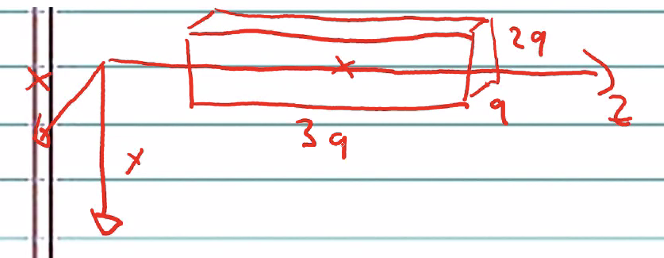
\includegraphics[scale=0.7]{Lecture-19/l19-img2.png}
\end{center}
We can write the inertia tensor to be diagonal:
\[\II = \m{I_1 & 0 & 0 \\ 0 & I_2 & 0 \\ 0 & 0 & I_3}\]
Where $I_1 > I_2 > I_3$ We can then have rotations around three possible axes:
\begin{center}
    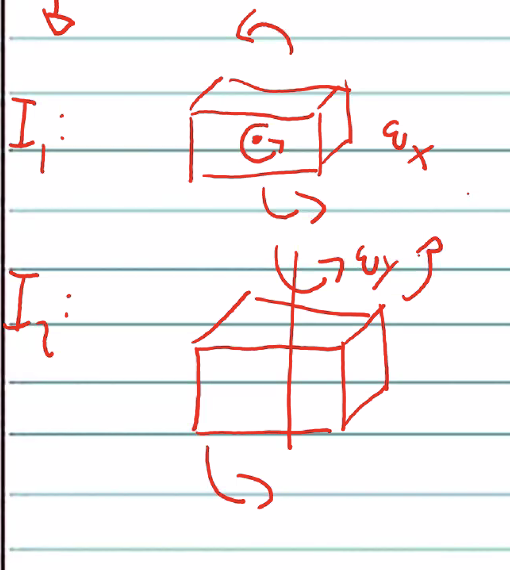
\includegraphics[scale=0.7]{Lecture-19/l19-img3.png}
    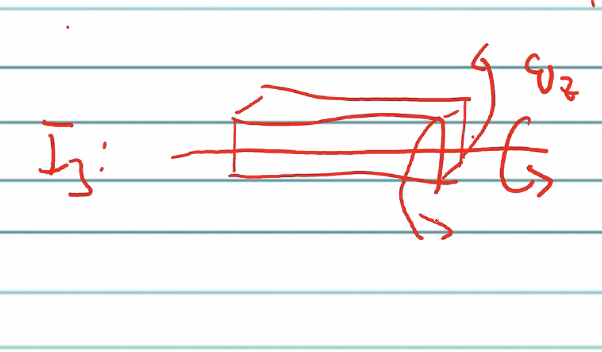
\includegraphics[scale=0.7]{Lecture-19/l19-img4.png}
\end{center}
We can now apply Euler's equations to learn something about this tumbling motion. Pick arbitrary axis (3) such that $\omega_3 \gg \omega_2 = \omega_1 \approx 0$, i.e. the body is rotating very fast about one axis and not the others. The Euler equations then give us:
\[\lambda_3\dot{\omega}_3 = (\lambda_1 - \lambda_2)\omega_1\omega_2 \approx 0\]
\[\lambda_1\dot{\omega}_1 = (\lambda_2 - \lambda_3)\omega_3\omega_2\]
\[\lambda_2\dot{\omega}_2 = (\lambda_3 - \lambda_1)\omega_3\omega_1\]
The first equation tells us that $\dot{\omega}_3 \approx 0$ and the angular velocity stays relatively constant. Let us take the time derivative of the second equation to learn more information:
\[\lambda_1\ddot{\omega}_1 = (\lambda_2 - \lambda_3)(\dot{\omega}_3\omega_2 + \omega_3\dot{\omega}_2)\]
By the first equation, $\dot{\omega}_3\omega_2 \approx 0$. We can therefore use the third equation to eliminate $\dot{\omega}_2$, which gives us:
\[\lambda_1 \ddot{\omega}_1 \approx (\lambda_2 - \lambda_3)\omega_3\frac{(\lambda_3 - \lambda_1)\omega_3\omega_1}{\lambda_2}\]
We can rewrite this as:
\[\ddot{\omega}_1 = -k\omega_1\]
Where
\[k = \frac{(\lambda_3 - \lambda_2)(\lambda_3 - \lambda_1)}{\lambda_1\lambda_2}\omega_3\]
This is a very familiar differential equation. The sign of $k$ will tell us about the resulting motion.
\newline (1) In the first case, suppose $\lambda_3 > \lambda_2$ and $\lambda_3 > \lambda_1$, or $\lambda_3 < \lambda_2$ and $\lambda_3 < \lambda_2$. In these two cases, we have that $k > 0$, and the above equation of motion for $\omega_1$ corresponds to simple harmonic motion (stable + oscillatory). 
\newline (2) In the second case, suppose $\lambda_1 < \lambda_3 < \lambda_2$ or $\lambda_2 < \lambda_3 < \lambda_1$, then $k$ is negative, and the above equation of motion for $\omega_1$ corresponds to real exponential solutions (unstable!)
\newline Our conclusion is that the rotation around the middle axis is unstable. This is a mathematical explanation for the famous intermediate axis theorem/tennis racket theorem, which we can see realized here: \\ \texttt{https://www.youtube.com/watch?v=1n-HMSCDYtM}